\documentclass[compress, aspectratio=32]{beamer}
\usepackage[utf8]{inputenc}
\usepackage{graphicx} % Required for inserting images
\graphicspath{ {./images/} }
\usepackage{amsmath}
\usepackage{mathspec}
\usepackage{xeCJK}
\usepackage{multicol}
\usepackage{float}
\usepackage{soul}
\usepackage{hyperref}
\usepackage{caption}
\usepackage{subcaption}
\usepackage{ulem}
\usepackage{listings}
\usepackage[backend=biber, citestyle=authoryear, sorting=none]{biblatex}
\addbibresource{ref.bib}

\useinnertheme{circles}
\useoutertheme[subsection=true, footline=authortitle]{miniframes}
%\usecolortheme{seagull}
\usefonttheme{structurebold}

\setmainfont{Sabon LT Pro}
\setsansfont{SF Pro Display}
%\setmathfont(Digits,Latin){Goldman Sans}
\setmonofont{IBM Plex Mono}

\AtBeginSection[]
{
    
  \begin{frame}[allowframebreaks]
    
    \tableofcontents[currentsection]
    
  \end{frame}
}

% \AtBeginSubsection[]{
%     \begin{frame}[allowframebreaks]
%         \tableofcontents[currentsubsection]
%     \end{frame}
% }

\title[Motors]{Driving Different Motors}
\subtitle{with Arduino}
\author{Ben Cheng}
\institute{RISD ID}
\date{\today}

\setbeamertemplate{navigation symbols}{\insertframenumber/\inserttotalframenumber}
\setbeamertemplate{title page}{
    \vbox{}
    \vfill
    \begin{beamercolorbox}[sep=8pt,left]{title}
        \begin{columns}
            \begin{column}[]{0.7\textwidth}
                \usebeamerfont{title}\inserttitle\par
        \ifx\insertsubtitle\@empty
        \else
          \vskip0.25em
          {\usebeamerfont{subtitle}\usebeamercolor[fg]{subtitle}\insertsubtitle\par}%
        \fi   
            \end{column}
            \begin{column}[]{0.1\textwidth}
                
\includegraphics[width=\textwidth]{IDSB-logo.png}
            \end{column}
        \end{columns}
          
      \end{beamercolorbox}
    \vskip1em\par
    \begin{beamercolorbox}[sep=8pt,left]{author}
      \usebeamerfont{author}\insertauthor
    \end{beamercolorbox}
    \begin{beamercolorbox}[sep=8pt,left]{institute}
        \usebeamerfont{institute}\insertinstitute
    \end{beamercolorbox}
    \begin{beamercolorbox}[sep=8pt,right]{date}
        \usebeamerfont{date}\insertdate
    \end{beamercolorbox}\vskip0.5em
    {\usebeamercolor[fg]{titlegraphic}\inserttitlegraphic\par}
    \vfill
}

\definecolor{customColor}{RGB}{90, 158, 108}
\setbeamercolor*{palette primary}{fg=customColor!60!black,bg=white!85!customColor}
\setbeamercolor*{palette secondary}{fg=customColor!70!black,bg=white!60!customColor}
\setbeamercolor*{palette tertiary}{bg=customColor!80!black,fg=white!50!customColor}
\setbeamercolor*{palette quaternary}{fg=customColor,bg=white!20!customColor}

\setbeamercolor*{sidebar}{fg=customColor,bg=customColor!75!white}

\setbeamercolor*{palette sidebar primary}{fg=customColor!10!black}
\setbeamercolor*{palette sidebar secondary}{fg=white}
\setbeamercolor*{palette sidebar tertiary}{fg=customColor!50!black}
\setbeamercolor*{palette sidebar quaternary}{fg=white!10!customColor}

\setbeamercolor*{titlelike}{parent=palette primary}
\setbeamercolor{frametitle}{bg=white!90!customColor}
\setbeamercolor{frametitle right}{bg=white!60!customColor}

\setbeamercolor{block title}{parent=palette tertiary}
\setbeamercolor{block body}{bg=white!90!customColor}

\setbeamercolor*{item projected}{parent=palette primary}%fg=black,bg=black!20}

\setbeamercolor*{normal text}{fg=black,bg=white}
\setbeamercolor*{alerted text}{fg=black}
\setbeamercolor*{example text}{fg=black}
\setbeamercolor*{structure}{fg=black}

\setbeamercolor{author in head/foot}{parent=title in head/foot}

\lstdefinestyle{mystyle}{basicstyle=\ttfamily\scriptsize, numbers=left, frame=lines, breaklines=true, showstringspaces=false}
\lstset{style=mystyle}

\begin{document}

\frame{\titlepage}

\begin{frame}[allowframebreaks]{Outline}
    \tableofcontents
\end{frame}

\section{Basic AC/DC Motor}
\subsection{Basics of Motors}
\begin{frame}
    \frametitle{Basic Principle of Motors}
    \begin{theorem}[Biot-Savart Law]
        \begin{equation*}
            \mathbf{B}=\frac{\mu_0}{4\pi}\oint_{C_1}\frac{I d \mathbf{I}^\prime \times \hat{\mathbf{R}}}{R^2}
        \end{equation*}
    \end{theorem}
    \begin{theorem}[Lorentz's equation]
        \begin{equation*}
            \mathbf{F}=q\mathbf{v}\times\mathbf{B}
        \end{equation*}
    \end{theorem}
\end{frame}

\begin{frame}
    \frametitle{AC vs DC Motors}
    \begin{figure}
        \centering
        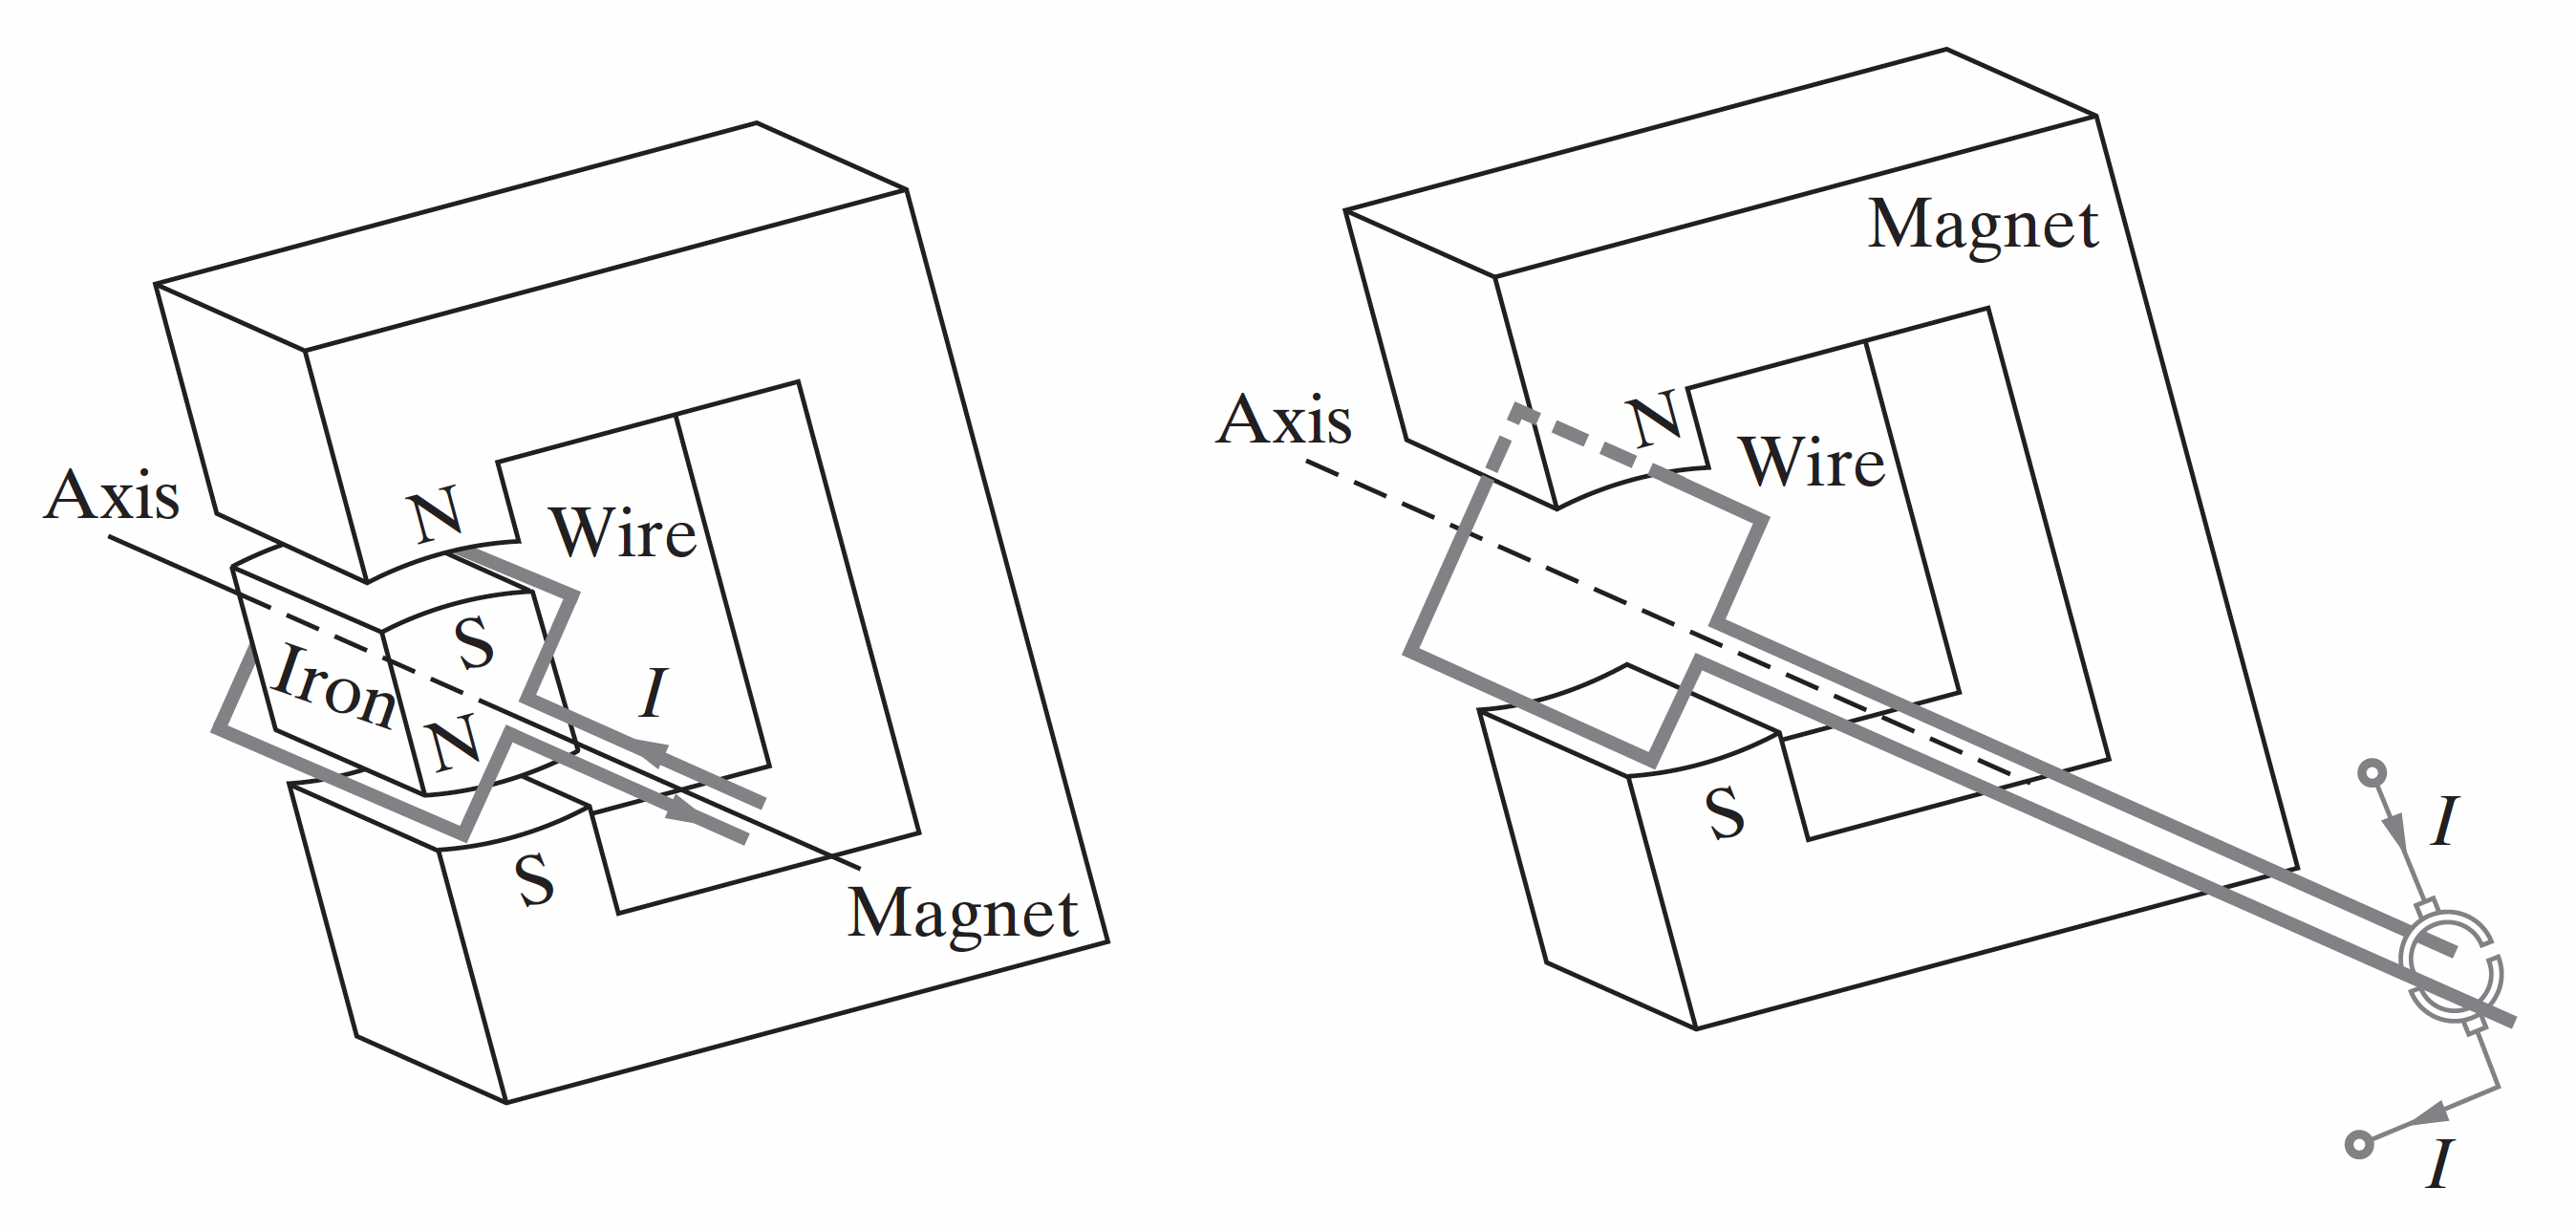
\includegraphics[width=0.8\textwidth]{motor.png}
        \caption{Simple dc motor. (Inan 2015)}
    \end{figure}
\end{frame}

\begin{frame}
    \frametitle{Torque and Power}
    \begin{columns}
        \begin{column}[]{0.5\textwidth}
            How much torque is needed to lift this?
            \begin{theorem}[Torque]
        \begin{equation*}
            \tau = F \times r
        \end{equation*}
        
    \end{theorem}
    
    \begin{figure}
        \centering
        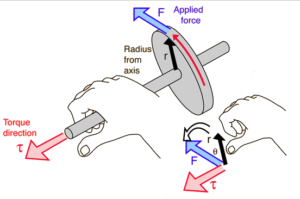
\includegraphics[height=0.3\textheight]{what-is-torque-300x199.jpg}
        \caption*{(Linear Motion Tips)}
    \end{figure}
    
        \end{column}
        \begin{column}[]{0.5\textwidth}
            How much power do I need to drive this motor?
            \begin{theorem}[Power]
                \begin{equation*}
                    P = I \times V
                \end{equation*}
                (Energy per unit time)
            \end{theorem}
            
        \end{column}
    \end{columns}
    
\end{frame}

\subsection{Analog Control}
\begin{frame}
    \frametitle{Analog Control}
    \begin{theorem}[Ohm's Law]
        \begin{equation*}
            V = A \times R
        \end{equation*}
        , or
        \begin{equation*}
            A = \frac{V}{R}
        \end{equation*}
    \end{theorem}
    \begin{itemize}
        \item Simple, accurate, predictable
        \item Power source = control unit
        \item Hard to implement on microcontroller
    \end{itemize}
\end{frame}

\subsection{Digital Control}
\begin{frame}
    \frametitle{Digital Control: PWM}
    \begin{columns}
        \begin{column}[]{0.5\textwidth}
            Pulse Width Modulation
            \begin{itemize}
                \item Easy to implement on microcontroller
                \item Easy manipulation
                \item Inaccurate approximation
                \item Power and control unit saperated
            \end{itemize}
        \end{column}
        \begin{column}[]{0.5\textwidth}
            \begin{figure}
        \centering
        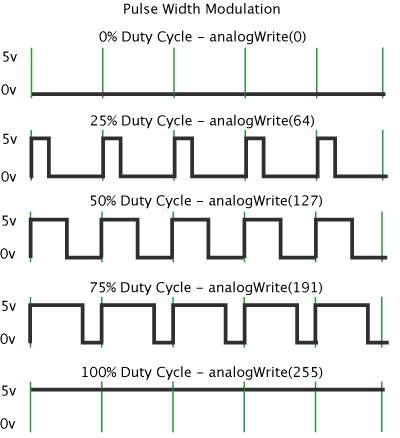
\includegraphics[height=0.7\textheight]{pwm.png}
        \caption*{(Arduino)}
    \end{figure}
        \end{column}
    \end{columns}    
\end{frame}

\begin{frame}
    \frametitle{PWM Approximation}
    \begin{figure}
        \centering
        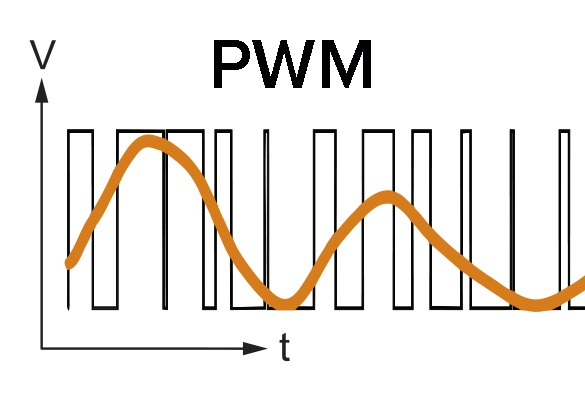
\includegraphics[height=0.7\textheight]{What-is-PWM-585x400.jpg}
        \caption*{(Thomson Linear)}
    \end{figure}
\end{frame}

\begin{frame}
    \frametitle{Saperated Power and Control Unit}
    \begin{columns}
        \begin{column}{0.4\textwidth}
            \begin{itemize}
                \item Scale of current:
                \begin{itemize}
                    \item $2A$: Fry a human
                    \item $0.35A$: DC Motor
                    \item $20mA$: Arduino Pinout
                \end{itemize}
                \item Saperate power and signal circuit
                \begin{itemize}
                    \item MOSFET
                    \item Bipolar Junction Transistor
                    \item Relay
                    \item H-Bridge
                \end{itemize}
            \end{itemize}
        \end{column}
        \begin{column}{0.6\textwidth}
            \begin{figure}
                \centering
                \includegraphics[width=0.6\textwidth]{Screenshot 2024-04-20 at 8.48.58 PM.png}
                \caption*{BJT. (Hambly 2018)}
            \end{figure}
        \end{column}
    \end{columns}
\end{frame}

\begin{frame}
    \frametitle{L298N Motor Driver}
    \begin{columns}
        \begin{column}{0.5\textwidth}
            \begin{figure}
                \centering
                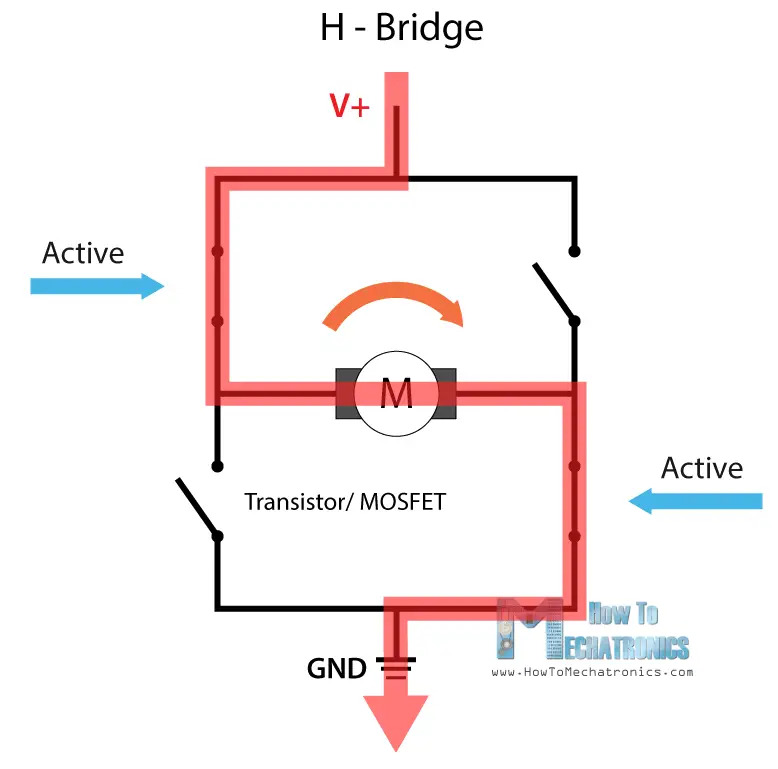
\includegraphics[height=0.7\textheight]{H-Bridge-configuration-How-It-Works.png.jpg}
                \caption*{(HowToMechatronics.com)}
            \end{figure}
        \end{column}
        \begin{column}{0.5\textwidth}
            \begin{itemize}
                \item ENA to pin 9 (PWM)
                \item IN1, IN2 to pin 5, 6
                \item GND and 12V to pwr supply
                \item OUT1, OUT2 to motor
            \end{itemize}
        \end{column}
    \end{columns}
\end{frame}

\begin{frame}[fragile]
    \frametitle{PWM Implementation}
    \begin{lstlisting}[language=c]
int speed = 255;
String inputStr = "";
bool clean = false;

void setup() {
    inputStr.reserve(200);
    Serial.begin(9600);
    // put your setup code here, to run once:
    pinMode(5, OUTPUT);
    pinMode(6, OUTPUT);
    pinMode(9, OUTPUT);

    digitalWrite(5, 1);
    digitalWrite(6, 0);
}

    \end{lstlisting}
\end{frame}

\begin{frame}[fragile]
    \frametitle{analogWrite()}
    \begin{lstlisting}[language=c]
void loop() {
    // put your main code here, to run repeatedly:
    if (clean) {
        analogWrite(9, inputStr.toInt());
        Serial.println(inputStr.toInt());
        // clear the string:
        inputStr = "";
        clean = false;
    }
    
    }
    \end{lstlisting}
\end{frame}

\section{Stepper Motor}
\begin{frame}
    \frametitle{Stepper Motor}
    \begin{figure}
        \centering
        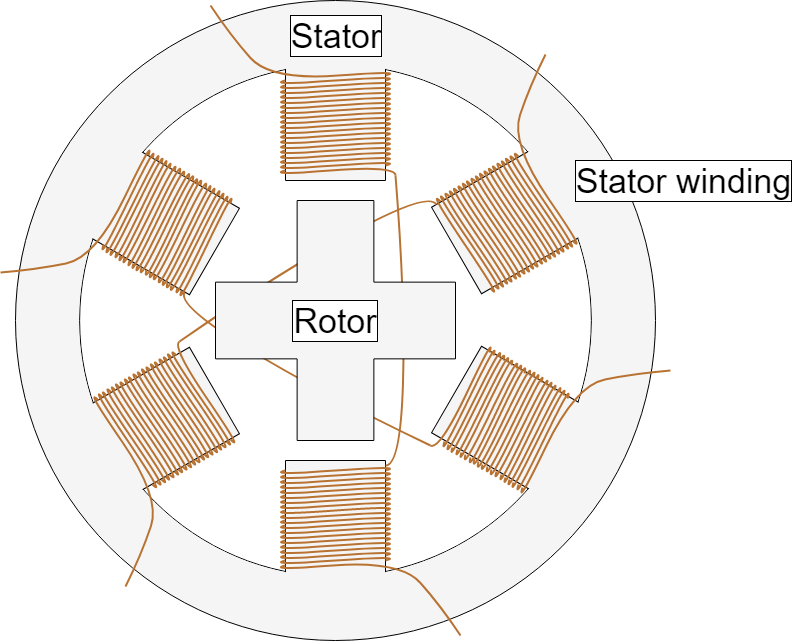
\includegraphics[height=0.7\textheight]{stepper.png}
        \caption*{(monolithicpower.com)}
    \end{figure}
\end{frame}
\begin{frame}
    \frametitle{28BYJ-48 Stepper Motor}
    \begin{columns}
        \begin{column}{0.5\textwidth}
           \begin{itemize}
        \item 4 coils
        \item 32 steps per revolution
        \item plus 64:1 gear ratio
        \item 2048 steps per revolution
        \item 5 pins
    \end{itemize} 
        \end{column}
        \begin{column}[]{0.5\textwidth}
            \begin{figure}
                \centering
                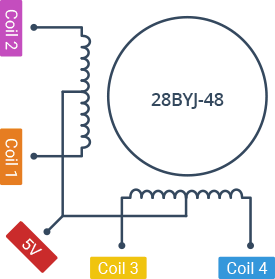
\includegraphics[width=0.6\textwidth]{28BYJ48-Stepper-Motor-Coil-Structure.png}
                \caption*{(lastminuteengineering.com)}
            \end{figure}
        \end{column}
    \end{columns}
    
\end{frame}
\begin{frame}
    \frametitle{Stepper vs DC Motor}
    \begin{itemize}
        \item Stepper is very accurate
        \item More difficult to control
        \item More power draw, more heat generation
        \item Stepper is suitable for short period, precise application.
        \item DC motor is for continuous, powerful application.
    \end{itemize}
\end{frame}

\begin{frame}
    \frametitle{ULN2003}
    \begin{columns}
        \begin{column}{0.5\textwidth}
            \begin{itemize}
                \item 7 Darlington pair (BJT)
                \item $500mA$ emitter current
            \end{itemize}
        \end{column}
        \begin{column}{0.5\textwidth}
            \begin{figure}
                \centering
                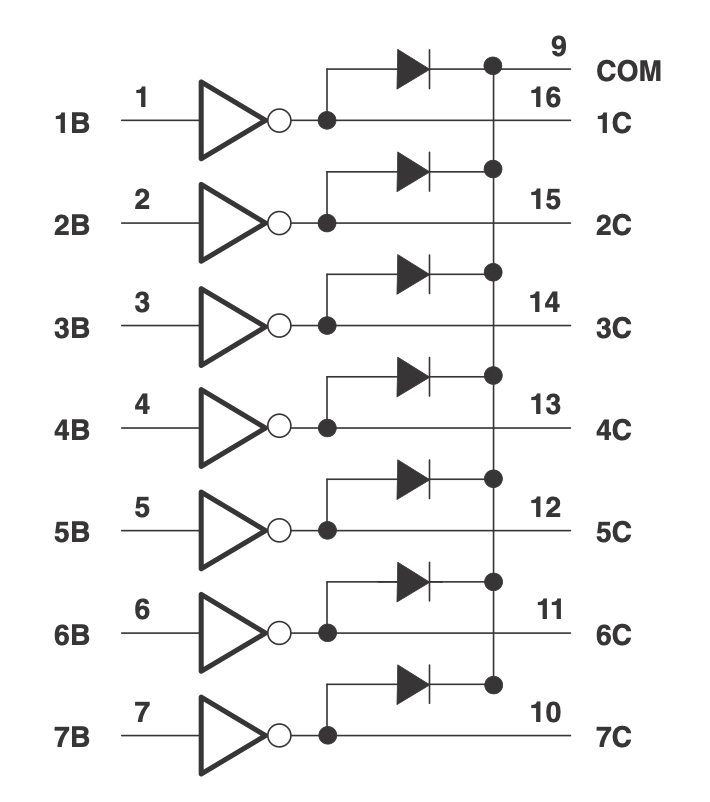
\includegraphics[height=0.7\textheight]{uln2003.png}
                \caption*{(Texas Instrument)}
            \end{figure}
        \end{column}
    \end{columns}
\end{frame}

\begin{frame}[fragile]
    \frametitle{Stepper Library}
    \begin{lstlisting}
#include <Stepper.h>

// initialize the stepper library on pins 8 through 11:
Stepper myStepper(stepsPerRevolution, 8, 9, 10, 11);

void setup() {
    // set the speed at 6 rpm:
    myStepper.setSpeed(6);
    // initialize the serial port:
    Serial.begin(9600);
}

void loop() {
    // step one revolution  in one direction:
    Serial.println("clockwise");
    myStepper.step(2048);
    delay(500);
}
    \end{lstlisting}
\end{frame}

\section{Servo Motor}
\begin{frame}
    \frametitle{Inside Servo Motor}
    \begin{columns}
        \begin{column}[]{0.5\textwidth}
           \begin{itemize}
        \item DC Motor
        \item Gearbox
        \item Encoder
        \item Controller IC
    \end{itemize} 
        \end{column}
        \begin{column}[]{0.5\textwidth}
            \begin{figure}
                \centering
                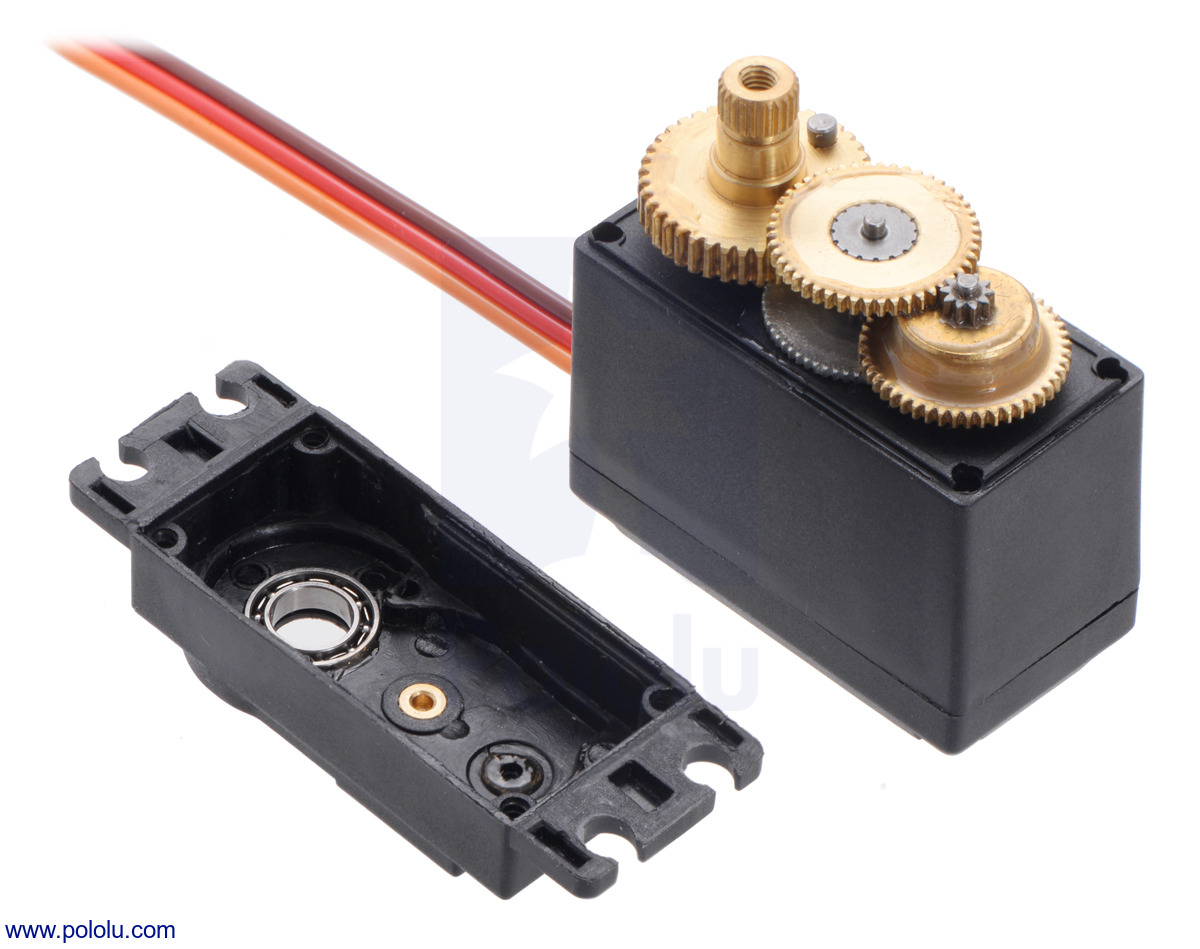
\includegraphics[width=0.8\textwidth]{servo fs5115m.jpeg}
                \caption*{(popolu.com)}
            \end{figure}
        \end{column}
    \end{columns}
    
\end{frame}
\begin{frame}
    \frametitle{Increasing Precision of DC Motor}
    \begin{figure}
        \centering
        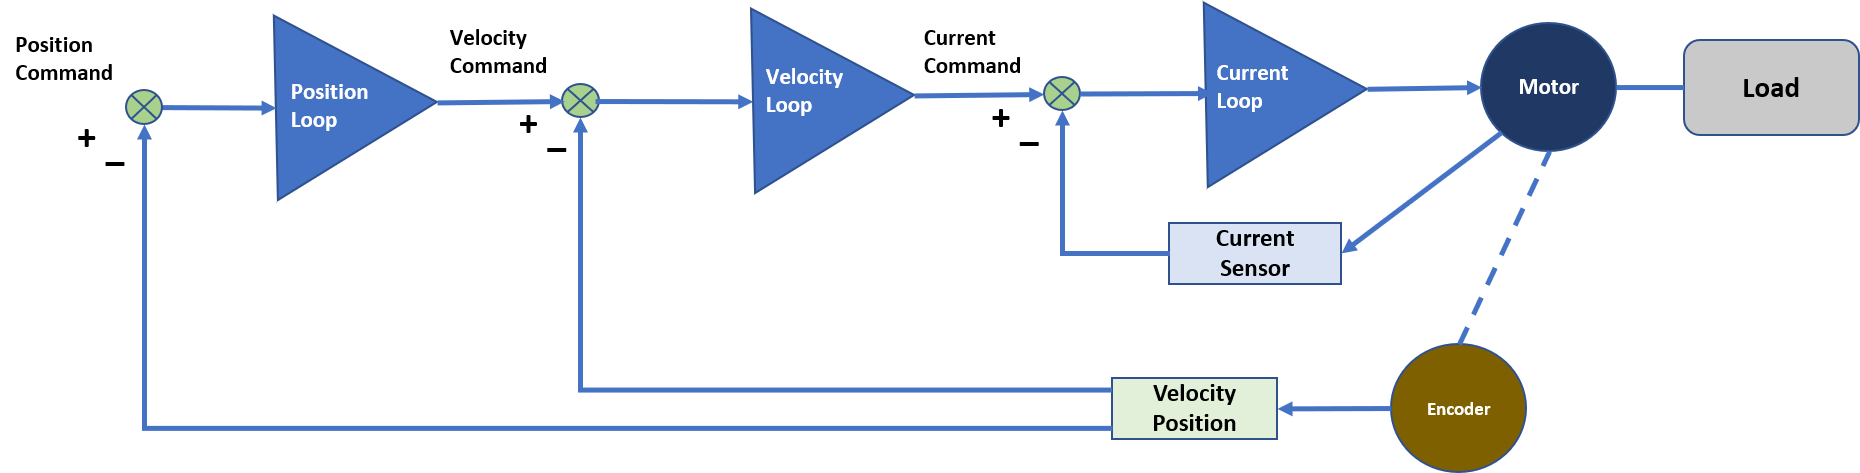
\includegraphics[width=\textwidth]{servo-motor-diagram-embedded-loops.jpg}
        \caption*{(Kollmorgan)}
    \end{figure}
\end{frame}

\begin{frame}[fragile]
    \frametitle{Sweep}
    \begin{itemize}
        \item Orange to pin 9, red to 3V3, brown to GND
    \end{itemize}
    \begin{lstlisting}[language=c]
#include <Servo.h>
Servo myservo;
void setup() {
    myservo.attach(9);
}
void loop() {
    int pos = 0;
    for (pos = 0; pos <= 180; pos += 1) {  
        myservo.write(pos);  
        delay(30);           
    }
    for (pos = 180; pos >= 0; pos -= 1) {  
        myservo.write(pos);                  
        delay(30);
    }
}
    \end{lstlisting}
\end{frame}
\begin{frame}
    \frametitle{Servo Pulse}
    \begin{figure}
        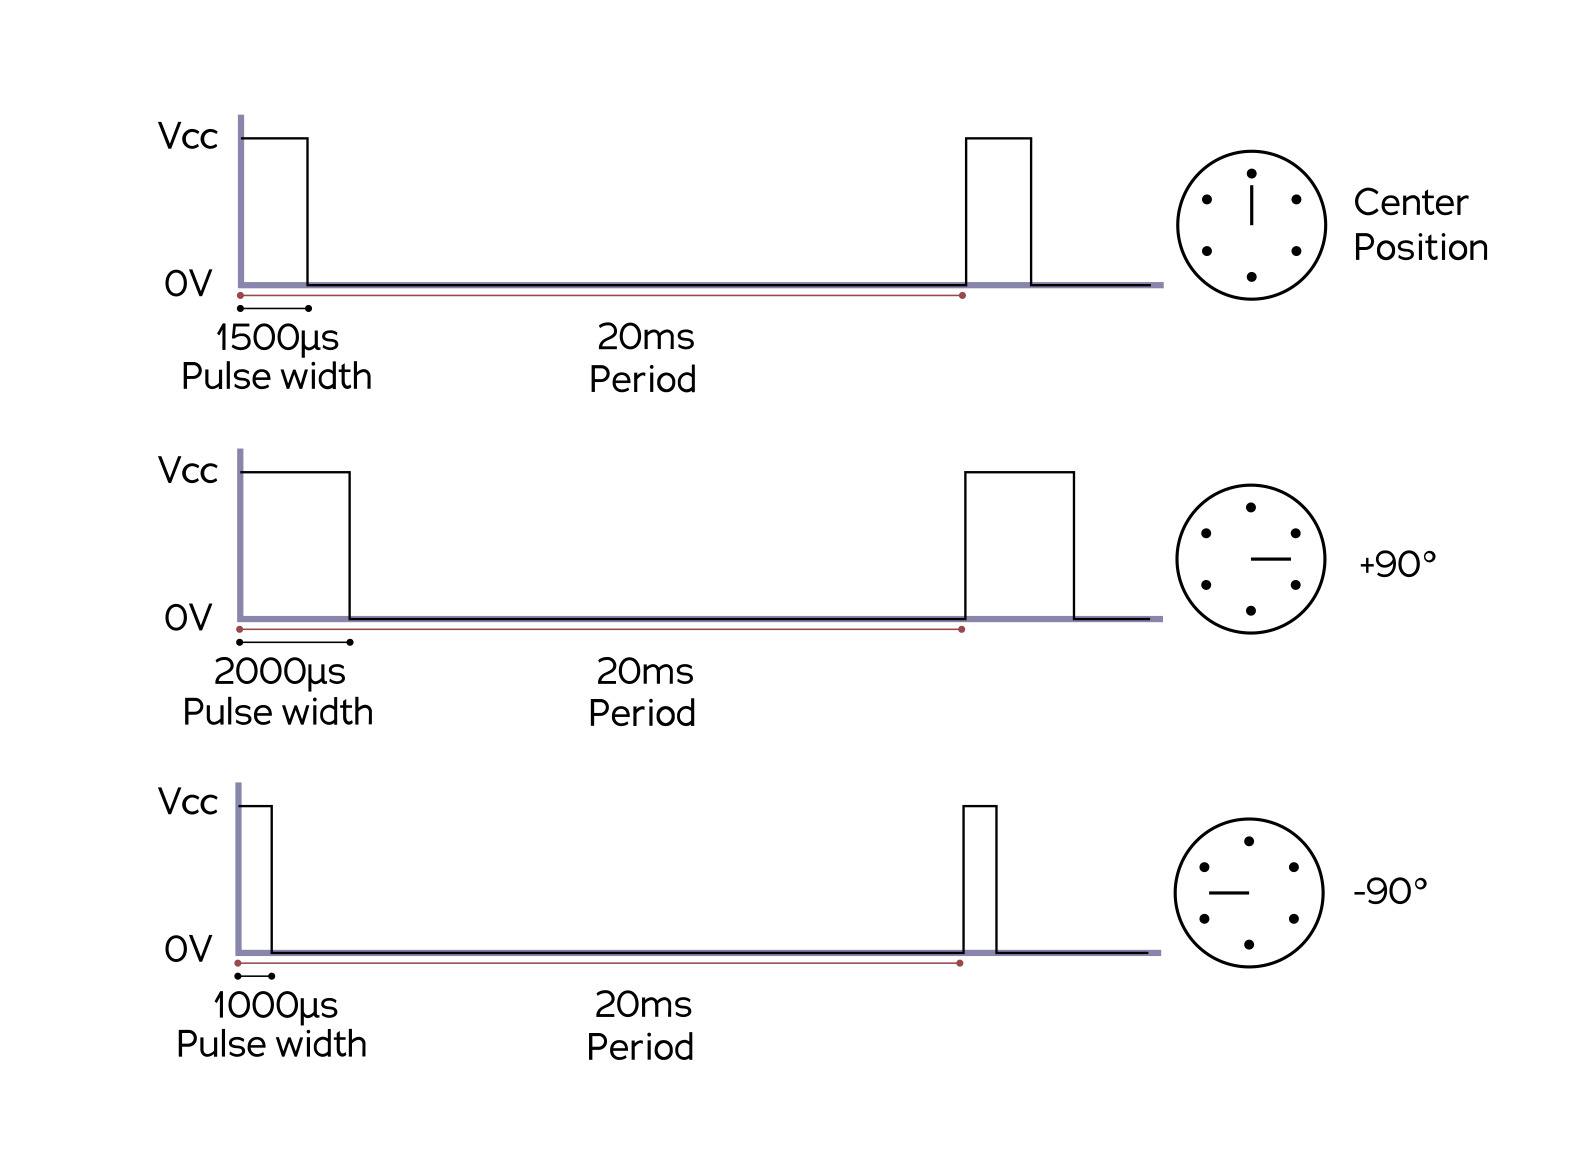
\includegraphics[height=0.7\textheight]{Servomotor_Timing_Diagram.jpg}  
        \centering
        \caption*{(Wikipedia user Hforesti)}
    \end{figure}
\end{frame}

\begin{frame}
    \frametitle{Servo vs Stepper vs DC Motor}
    \begin{columns}
        \begin{column}[]{0.3\textwidth}
            Servo
            \begin{itemize}
                \item precise
                \item digital
                \item for less than 1 rev
            \end{itemize}
        \end{column}
        \begin{column}[]{0.3\textwidth}
            Stepper
            \begin{itemize}
                \item precise
                \item digital
                \item for short period
            \end{itemize}
        \end{column}
        \begin{column}[]{0.3\textwidth}
            Servo
            \begin{itemize}
                \item not for angular precision
                \item digital/analog
                \item for continuous rev
            \end{itemize}
        \end{column}
    \end{columns}
\end{frame}
\end{document}